% ---------------------------------------------------------------------
% HEADER
% Formålet med å legge header til et eget dokument er å garantere at
% oppsettet av dokumentene er likt for alle løsningsforslagene.
% I headeren skjer følgende:
% (1) Dokumentet blir startet
% (2) Pakker blir importert
% ---------------------------------------------------------------------
% ---------------------------------------------------------------------
% HEADER
% Formålet med header er å importere de samme pakkene i alle dokumentene.
% ---------------------------------------------------------------------

% Sett opp dokumentet. Her kan 'twoside' brukes for printing
\documentclass[12pt, a4paper]{article}

% Vi trenger utf-8 for å bruke norske bokstaver: Æ, Ø, Å
\usepackage[utf8]{inputenc}

% Vi setter babel til norsk, da får dokumentegenskaper norske titler
\usepackage[norsk]{babel}

% For å kunne bruke grafikk
\usepackage{graphicx}
\newcommand{\figwidth}{0.75}

% Matematikkpakker fra AMS - American Mathematical Society
\usepackage{amsmath, amsthm, amsfonts, amssymb, mathtools}

% For eventuelle linker, e.g. \href{URL}{text}
\usepackage{hyperref}

% For headers og footers med eventuell logo
\usepackage{fancyhdr}

% Sett marginer manuelt
\usepackage[top = 3cm, left = 3cm, right = 3cm, bottom = 3cm]{geometry}

% For enkle lister, nyttig for oppgave a), b), c), ...
\usepackage[sharp]{easylist}

% Dersom flere kolonner er ønskelig i deler av dokumentet
\usepackage{multicol}

% For luft mellom paragrafer
\usepackage{parskip}

% For logikk assosiert med logoer
\usepackage{ifthen}

% For å finne totalt antall sider
\usepackage{lastpage}

% Annet
\usepackage{enumitem}

\usepackage{polynom}% Polynomer
\polyset{style=C, div=:}

\usepackage{systeme}% Likningssystemer

% Kan brukes når noe stryker ut noe, f.eks 1/n * n, her kan man ta \frac{1}{\cancel{n}} * \cancel{n}
\usepackage{cancel}



% ---------------------------------------------------------------------
% DOKUMENTVARIABLER
% ---------------------------------------------------------------------
\newcommand{\fagkode}{S2}
\newcommand{\semesteraar}{høsten 2017}
\newcommand{\forfatter}{Tommy O.}
\newcommand{\dokumenttittel}{Løsningsforslag -- Eksamen \fagkode, \semesteraar}


% Set til 'true' og oppgi logo dersom du vil bruke en logo
\newboolean{bruklogo}
\setboolean{bruklogo}{false}
\newcommand{\logonavn}

% ---------------------------------------------------------------------
% SETUP
% Formålet med å legge setup til et eget dokument å garantere at headers,
% footers, og øverste del av dokumentet er likt for alle
% løsningsforslagene.
% ---------------------------------------------------------------------
% ---------------------------------------------------------------------
% HEADER
% Formålet med setup er at dokumentene ser rimelig like ut.
% ---------------------------------------------------------------------


% ---------------------------------------------------------------------
% Alternativ font. Kommentert ut fordi Computer Modern (default) er pen
%\usepackage{kmath,kerkis}
%\usepackage[T1]{fontenc}
% ---------------------------------------------------------------------


% ---------------------------------------------------------------------
% Sett opp headers og footers
\ifthenelse{\boolean{bruklogo}}{
% Dersom logo skal brukes, sett logoen oppe til høyre med bredde 4 cm
	\rhead{\includegraphics[width=3.5cm]{\logonavn}}
}{
% Dersom logo ikke skal brukes, sett tom header
	\rhead{}
} 
\rfoot{\thepage}
\cfoot{}
\lhead{}
\lfoot{{\scriptsize Forbedringsforslag? Bidra på \url{https://github.com/tommyod/matte_eksamener_VGS}.}}
\renewcommand{\headrulewidth}{0pt}
% ---------------------------------------------------------------------


% ---------------------------------------------------------------------
% To streker under svaret
\def\answer#1{\underline{\underline{#1}}}
% ---------------------------------------------------------------------


% ---------------------------------------------------------------------
% Start selve dokumentet
% ---------------------------------------------------------------------

\begin{document}
\pagestyle{fancy}
{\bfseries \Large \dokumenttittel} \\
{ \footnotesize Laget av \forfatter 
	\hfill Sist oppdatert: \today 
	\hfill Antall sider: \pageref*{LastPage}}
\hrule
\vspace{1em}
\begin{center}
\fbox{\fbox{\parbox{.90\textwidth}{
	Dette dokumentet er open-source;
	alle kan bidra til å gjøre det bedre.
	Dersom du finner skrivefeil, matematiske feil, eller ser at forklaringene kan være bedre: ikke nøl med å sende inn en endring. 
	Du kan finne siste versjon, og bidra, på GitHub, se:
	\url{https://github.com/tommyod/matte_eksamener_VGS}
}}}
\end{center}


% ---------------------------------------------------------------------
% DOKUMENTSTART - Skriv løsningsforslaget nedenfor
% ---------------------------------------------------------------------	
\section*{Del 1 - uten hjelpemidler}
\subsection*{Oppgave 1}
\begin{easylist}[enumerate]
\ListProperties(Style2*=,Numbers=a,Numbers1=l,FinalMark={)})
# Vi skal derivere $f(x) = 2x^2 - 4x^3$.
Vi bruker regelen
\begin{equation*}
	(af(x) + bg(x))' = a f'(x) + b g'(x),
\end{equation*}
samt regelen $(x^n)' = nx^{n-1}$ og får
\begin{align*}
	f'(x) &= \left[ 2x^2 \right]' - \left[ 4x^3\right]' = 
	2\left[ x^2 \right]' - 4 \left[x^3 \right]' \\ 
	&= 2\left[ 2 x^1 \right] - 4 \left[3 x^2 \right] = 
	4x - 12 x^2 = \answer{4x (1 - 3x)}.
\end{align*}

# Vi skal derivere $g(x) = x^2 e^x$, og vi må her bruke produktregelen $(uv)' = u'v + uv'$. Det kan være greit å regne ut følgende på forhånd.
\begin{align*}
	u(x) = x^2 \quad & u'(x) = 2x \quad \\ 
	v(x) = e^x \quad & v'(x) = e^x \quad 
\end{align*}
Svaret blir da
\begin{equation*}
	f'(x) = u'v + uv' = 2x e^x + x^2e^x = \answer{xe^x (x + 2)}.
\end{equation*}

# Vi skal derivere $h(x) = \ln \left(x^3 + 3x + 1\right)$.
Her må vi bruke kjerneregelen, som sier at $f'(x) = f'(u) u'(x)$.
Her er $u(x) = x^3 + 3x + 1$ og $u'(x) = 3x^2 + 3$, vi får
\begin{equation*}
	f'(x) = f'(u) u'(x) = \left( \ln (u)\right)' u'(x) = \frac{1}{u} u'(x) =
	\frac{3x^2 + 3}{x^3 + 3x + 1} = \answer{\frac{3(x^2 + 1)}{x^3 + 3x + 1}}.
\end{equation*}
\end{easylist}

\subsection*{Oppgave 2}
\begin{easylist}[enumerate]
\ListProperties(Style2*=,Numbers=a,Numbers1=l,FinalMark={)})
# Vi bruker polynomdivisjon som vanlig.
\begin{center}
	\polylongdiv{x^3 - 5x^2 - 4x + 20}{x - 5}
\end{center}
Svaret blir altså $\answer{x^2 - 4}$.


# Generelt så vet vi at dersom $p(t) \div (x - a)$ går opp, så må $p(a)$ være lik $ 0$.
Her er $a = -1$, så vi setter opp likningen $p(-1) = 0$ og løser slik:
\begin{align*}
	p(x = -1) = (-1)^3 + t(-1)^2 + 5(-1) - 2t &= 0 \\
	 -1 + t + -5 - 2t &= 0 \\
	 -t - 6 &= 0 \\
	  t &= -6.
\end{align*}
Divisjonen går opp når \answer{$t = -6$}.
\end{easylist}

\subsection*{Oppgave 3}
Det finnes flere måter å løse likningssystemer på.
Metoden jeg bruker nedenfor heter Gauss-eliminasjon, og er en rimelig enkel, strukturert måte å gjøre det på. 
Idéen er å lage nuller nede til venstre i likningsystemet, og deretter ``løse oppover.''
Vi skal løse systemet:
\begin{align*}
	A:& \quad x  +   y  +  2z = -3 \\
	B:& \quad x  +    3y  +   z = 2 \\
	C:& \quad 2x   +  y  +   z = 2 .
\end{align*}
Vi setter $B_1 = B - A$ og $C_1 = C - 2A$, da får vi:
\begin{align*}
A:& \quad x  +   y  +  2z = -3 \\
B_1:& \quad \mathbf{0}x  +    2y     -z = 5 \\
C_1:& \quad \mathbf{0}x   -  y    -3z = 8
\end{align*}
Vi setter så $C_2 = C_1 + B_1 / 2$ og får:
\begin{align*}
A:& \quad x  +   y  +  2z = -3 \\
B_1:& \quad \mathbf{0}x  +    2y     -z = 5 \\
C_2:& \quad \mathbf{0}x   -  \mathbf{0}y    -\frac{7}{2}z = \frac{21}{2}
\end{align*}
Først løser vi likning $C_2$ for $z$ og får \answer{$z = -3$}.
Deretter løser vi likning $B_1$ for $y$ og får \answer{$y = 1$}.
Til slutt løser vi likning $A$ for $x$ og får \answer{$x = 2$}.
Denne teknikken heter Gauss-eliminasjon, den gjør først systemet \emph{triangulært} ved å lage nuller nede til venstre, og deretter løser man oppover.
Vi kan også løse ved innsetingsmetoden, eller bruke addisjonsmetoden uten å nødvendigvis gjøre systemet triangulært.
Uansett hva vi gjør bør vi sette inn $x$, $y$ og $z$ i likningene og sjekke at svaret stemmer.


\subsection*{Oppgave 4}
Her bruke vi logaritmesetningene, og vi får
\begin{align*}
	\ln \left(\frac{e^2}{2}\right) + 2 \ln (2) - \ln \left(\frac{2}{e^4}\right) &=  \\
	\ln(e^2) - \ln(2) + 2\ln(2) - \left( \ln (2) - \ln (e^4)\right) &= \\
	2 \ln(e) - \ln(2) + 2\ln(2) - \ln (2) + 4 \ln (e) &= \\
	6 \ln(e) &= \answer{6} .
\end{align*}

\subsection*{Oppgave 5}
\begin{easylist}[enumerate]
\ListProperties(Style2*=,Numbers=a,Numbers1=l,FinalMark={)})
# Generelt i en aritmetisk rekke så er $a_n = a_1 + d(n-1)$,
der $d$ er en konstant differanse mellom leddene $a_i$ og $a_{i+1}$.
Vi ser at $d = 4$, så vi får
\begin{equation*}
	a_n = a_1 + d(n-1) =  3 + 4(n-1) = \answer{4n - 1}.
\end{equation*}
På eksamen er det lurt å verifisere at svaret stemmer med å regne ut $a_1$, $a_2$ og $a_3$. 
Vi kan sjekke at vi får $a_1 = 3$, $a_2 = 7$ og $a_3 = 11$---da kan vi være rimelig sikre på at svaret er riktig.

# Vi ønsker å bruke summeformelen for en artimetisk rekke.
For å bruke denne må vi finne $a_1$, $a_n$ og $n$.
Vi vet allerede at $a_1 = 3$ og $a_n = 119$.
For å finne $n$ bruker vi formelen $a_n = a_1 + d(n-1)$.
Vi får at
\begin{equation*}
	a_n = a_1 + d(n-1) \quad \Rightarrow  \quad
	119 = 3 + 4(n-1) \quad \Rightarrow \quad n = 30.
\end{equation*}
Deretter er det bare å sette inn i formelen for sum av en artimetisk rekke og regne ut.
\begin{equation*}
	S_n = \frac{(a_1 + a_n) n}{2} = \frac{(3 + 119) 30}{2} = \frac{122 \cdot 30}{2} = 61 \cdot 30 = \answer{1830}.
\end{equation*}
\end{easylist}


\subsection*{Oppgave 6}
Vi ser på funksjonen $K(x) = x^2 + 50x + 6400$.
\begin{easylist}[enumerate]
\ListProperties(Style2*=,Numbers=a,Numbers1=l,FinalMark={)})
# Grensekostnaden er den deriverte av $K(x)$. 
Vi regner enkelt ut at $K'(x) = 2x + 50$, og da blir $K'(50) = 2 (50) + 50 = \answer{150}$.
Funksjonen $K(x)$ er total kostnad per uke når $x$ enheter blir produsert.
Da er grensekostnaden $K'(x)$ endringen i kostnaden per endring i enheter $x$.
At $K'(50) = 150$ betyr at dersom bedriften ønsker å gå fra å produsere $50$ til å produsere $51$ enheter per uke, vil totalkostnaden øke med omtrent $150$.

# Kostnad per enhet er $G(x) = K(x)  / x$.
Vi finner verdien som gir minimal verdi for denne funksjonen
ved å derivere og sette lik null. Vi har at 
\begin{equation*}
	G(x) = \frac{K(x)}{x} = \frac{x^2 + 50x + 6400}{x} = x + 50 + \frac{6400}{x}.
\end{equation*}
Vi husker at $1 / x = x^{-1}$, deriverer, og setter lik null slik at vi får
\begin{equation*}
G'(x) = 1 - \frac{6400}{x^2} = 0.
\end{equation*}
Dette gir likningen $x^2 = 6400$, som har positiv løsning \answer{$x = 80$}.
Vi ser bort i fra den negative løsningen ettersom negativ produksjonsmengde ikke gir mening.
Produksjonsmengden som gir lavest kostnad per produserte enhet er $80$.
\end{easylist}

\subsection*{Oppgave 7}
Vi skal studere funksjonen
\begin{equation*}
	f(x) = (x - 2) e^x,
\end{equation*}
og det kan være lurt å regne ut den deriverte og den dobbelderiverte med en gang.
Med flittig bruk av produktregelen får vi at
\begin{equation*}
	f'(x) = (x - 1) e^x \quad \text{og} \quad f''(x) = x e^x.
\end{equation*}

\begin{easylist}[enumerate]
\ListProperties(Style2*=,Numbers=a,Numbers1=l,FinalMark={)})
# Nullpunkt oppstår når $f(x) = 0$. Vi må løse
\begin{equation*}
	f(x) = (x - 2) \underset{\text{alltid } > 0}{\underbrace{e^x}} = 0,
\end{equation*}
og ettersom $e^x > 0$ for alle verdier av $x$ så er $f(x) = 0$ når $(x-2) = 0$.
Da er \answer{$x = 2$ et nullpunkt}.
Funksjonen har ingen andre nullpunkter.

# Stasjonære punkt oppstår når $f'(x) = 0$. Vi må løse
\begin{equation*}
f'(x) = (x - 1) \underset{\text{alltid } > 0}{\underbrace{e^x}} = 0,
\end{equation*}
og ettersom $e^x > 0$ for alle verdier av $x$ så er $f'(x) = 0$ når $(x-1) = 0$.
Et stasjonært punkt oppstår når $x = 1$, da er 
\begin{equation*}
	y = f(1) = ((1) - 2) e^1 = -e.
\end{equation*}
Punktet \answer{$(x, y) = (1, -e)$} er et stasjonært punkt.
Det er et \answer{bunnpunkt}, det kan vises på 2 forskjellige måter:
## Andrederiverttesten. $f''(1) = 1 e^1 = e > 0$, da er $x = 1$ et bunnpunkt.
## Fortegnslinje. Vi lager en fortegnslinje for $f'(x)$ slik
\begin{center}
	
\includegraphics[width=0.65\linewidth]{figs/fortegn2.pdf}
\end{center}
Vi ser at $f'(x)$ er negativ til venstre for $x = 1$ og positiv til høyre for $x = 1$, da må punktet være et bunnpunkt.

# Vendepunkt oppstår når $f''(x) = 0$. Vi må løse
\begin{equation*}
f''(x) = x \underset{\text{alltid } > 0}{\underbrace{e^x}} = 0,
\end{equation*}
og ettersom $e^x > 0$ for alle verdier av $x$ så er $f(x) = 0$ bare når $x = 0$.
Et vendepunkt oppstår altså når $x = 0$, da er 
\begin{equation*}
y = f(0) = (0 - 2) e^0 = -2.
\end{equation*}
Punktet \answer{$(x, y) = (0, -2)$} er et vendepunkt.


# Funksjonen er skissert nedenfor.
På eksamen er det nok best å lage en tabell, samt å bruke det man vet om monotoniegenskaper og vendepunkt, til å lage en skisse.
\begin{center}
	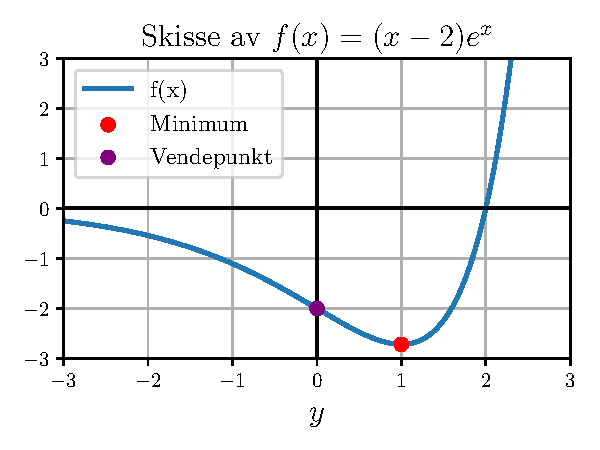
\includegraphics[width=0.55\linewidth]{code/oppg_7d.pdf}
\end{center}


\end{easylist}

\subsection*{Oppgave 8}
Nettogevinsten regnes ut ved å ta utbetalt gevinst minus prisen av loddet.
Vi lager en tabell der første rad er de mulige utfallene i utfallsrommet, og andre rad er sannsynligheten for de forskjellige utfallene.
\begin{center}
	\begin{tabular}{|c|c|c|c|} \hline
		$x$ & 0 & 40 & -10 \\ \hline
		$P(X = x)$ & 0.5 & 0.1 & 0.4  \\ \hline
	\end{tabular}
\end{center}
\begin{easylist}[enumerate]
\ListProperties(Style2*=,Numbers=a,Numbers1=l,FinalMark={)})
# Definisjonen av $\operatorname{E}(X)$ er $\operatorname{E}(X) = \sum_{x \in X}P(X = x)x$, og vi får
\begin{equation*}
\operatorname{E}(X) = \sum_{x \in X}P(X = x)x =  0 (0.5) + 40 (0.1) -10 (0.4) = 4 - 4 = \answer{0}.
\end{equation*}

Generelt er likningen for varians gitt ved:
\begin{equation*}
\operatorname{Var}(X) = \sum_{x \in X}P(X = x)(x - \operatorname{E}(X))^2 
\end{equation*}
Ettersom $\operatorname{E}(X) = 0$ får vi en rimelig enkel utregning:
\begin{align*}
\operatorname{Var}(X) &= \sum_{x \in X}P(X = x)x^2 \\
&= 0.5 (0 - 0)^2 + 0.1 (40 - 0)^2 + 0.4 (-10 - 0)^2 \\
&= 0 + 0.1 (1600) + 0.4 (100) = 160 + 40 = \answer{200}
\end{align*}
# Sentralgrenseteoremet sier at dersom $X_1, X_2, \dots, X_n$ er stokastiske variabler så vil summen
\begin{equation}
	\label{eqn:sentral}
	S_n = X_1 + X_2 + \dots + X_n
\end{equation}
bli normalfordelt når $n \to \infty$. 
Her går ikke $n$ til evig, men $n = 50$ er stor nok til å anta at summen er normalfordelt.
Se figur \ref{fig:oppg_8b} for en visualisering av hvordan summen blir normalfordelt på grunn av sentralgrenseteoremet.

\begin{figure}[ht!]
\centering
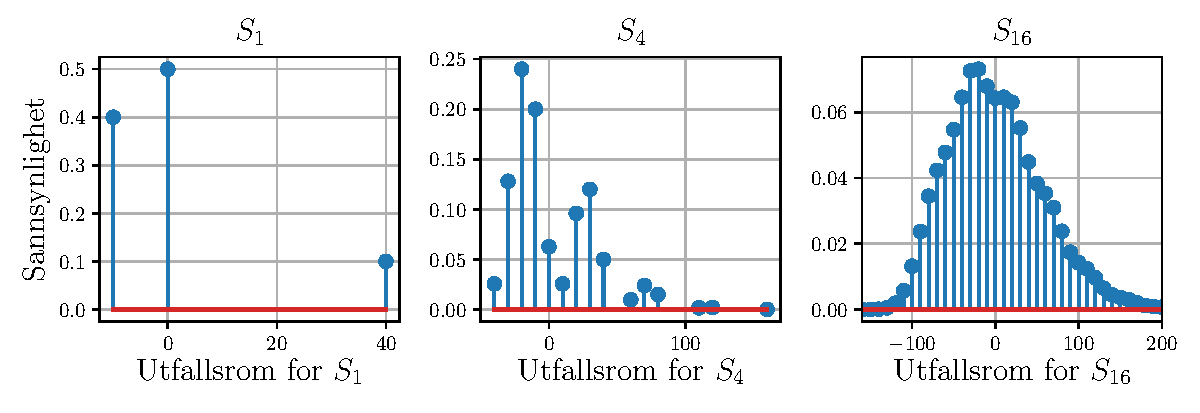
\includegraphics[width=0.99\linewidth]{code/oppg_8b.pdf}
\caption{Utfallsrom og sannsynligheter for $S_1 = X$, $S_4$ og $S_{16}$ fra likning \eqref{eqn:sentral}.
	I utfallsrommet til $S_1$ ser vi de tre utfallene $\left\{-10, 0, 40\right\}$ tydelig, samt de tilhørende sannsynlighetene. 
	Utfallsrommet til $S_4$ er større fordi det er flere muligheter. Vi kan se at beste utfall er $160$, altså å få nettogevist på 40 kroner 4 ganger på rad---sannsynligheten for dette er liten.
	Utfallsrommet til $S_{16}$ begynner å ligne normaltfordelt, og sentralgrenseteoremet sier at $S_n$ blir normaltfordelt når $n$ går mot evig.}
\label{fig:oppg_8b}
\end{figure}



# Vi gjør følgende utregning for forventningsverdien.
\begin{align*}
	\operatorname{E}(S) &= \operatorname{E}(X_1 + X_2 + \dots + X_{50}) \\
	&= \operatorname{E}(X_1) + \operatorname{E}(X_2) + \dots + \operatorname{E}(X_{50}) \\
	&= 0 + 0 + \dots + 0 = \answer{0}
\end{align*}
Vi gjør samme type utregning for variansen.
\begin{align*}
\operatorname{Var}(S) &= \operatorname{Var}(X_1 + X_2 + \dots + X_{50}) \\
&= \operatorname{Var}(X_1) + \operatorname{Var}(X_2) + \dots + \operatorname{Var}(X_{50}) \\
&= 200 + 200 + \dots + 200 = 50 (200) = 10000
\end{align*}
Ettersom $\operatorname{SD}(S) = \sqrt{\operatorname{Var}(S)}$ får vi at $\answer{\operatorname{SD}(S) = \sqrt{10000} = 100}$.
# Dersom Anja satser 500 kroner så har hun råd til 50 lodd.
Dersom hun skal få råd til en jakke som koster 650 kroner må nettogevinsten
være minst 150 kroner. Vi må finne $P(S \geq 150)$, og det gjør vi slik:
\begin{align*}
	P(S \geq 150) &= 1 - P(S < 150) \\
	&= 1 - P\left( \frac{S - \mu}{\sigma} < \frac{150 - \mu}{\sigma}\right) \\
	&= 1 - P\left( Z < \frac{150 - 0}{100}\right) \\
	&= 1 - P\left( Z < 1.5\right) \\
	&= 1 - 0.9332 \quad \text{(fra Vedlegg 1, ``Standard normalfordeling'')} \\
	&= \answer{0.067 = 6.7 \%}
\end{align*}
Sannsynligheten for at Anja får nok penger til å kjøpe jakken er $6.7 \%$.
\end{easylist}



\section*{Del 2 - med hjelpemidler}

\subsection*{Oppgave 1}
\begin{easylist}[enumerate]
\ListProperties(Style2*=,Numbers=a,Numbers1=l,FinalMark={)})
# Vi bruker \verb|Funksjon( <Funksjon>, <Start>, <Slutt> )| i Geogebra.
Se figur \ref{fig:H17_del2_1a} for resultatet.
\begin{figure}[ht!]
	\centering
	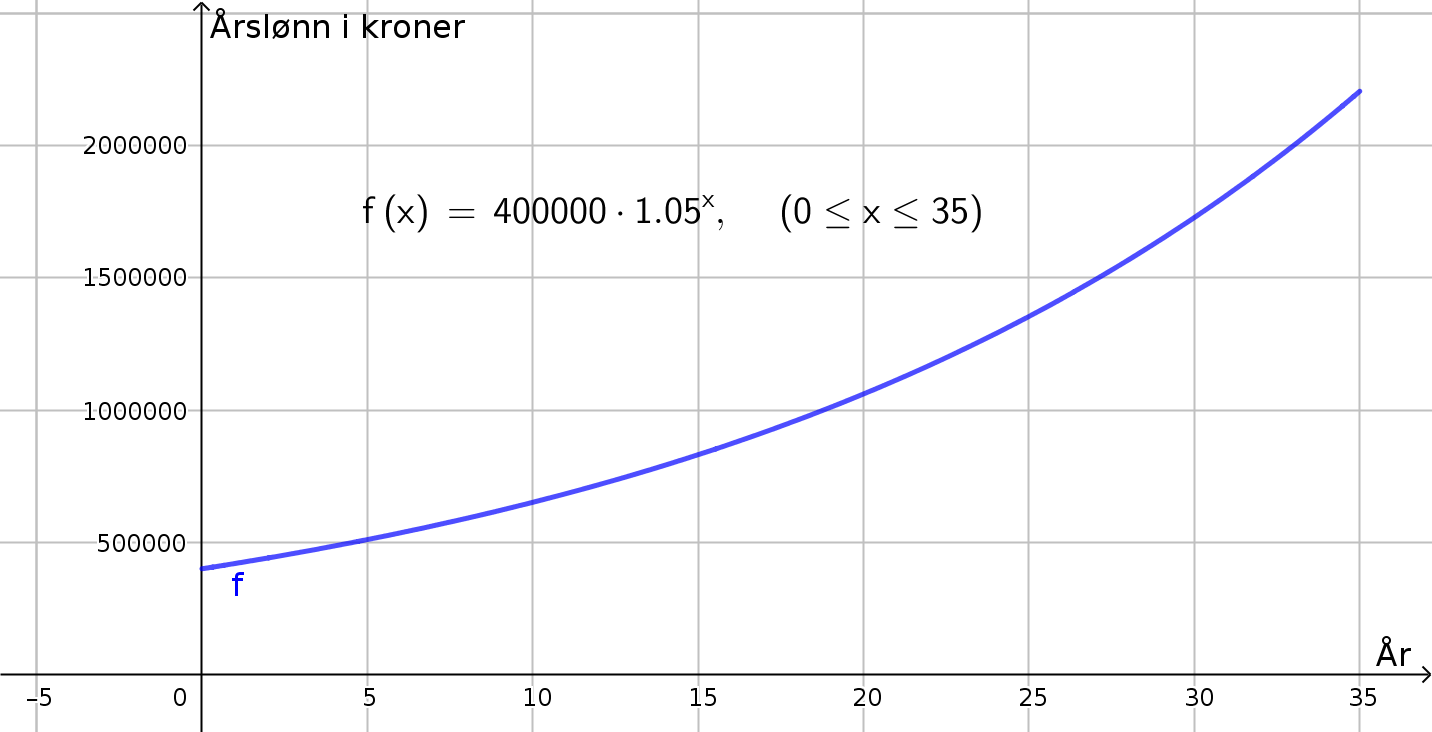
\includegraphics[width=0.70\linewidth]{figs/H17_del2_1a}
	\caption{Grafen $f(x) = 400000 \times 1.05^x$ tegnet i Geogebra for $0 \leq x \leq 35$.}
	\label{fig:H17_del2_1a}
\end{figure}
# Vi løser $f(x) = 800000$ for $x$.
Svaret blir $x = 14.21$, se figur \ref{fig:H17_del2_1bcde}.
Her må vi gjøre en tolkning.
I virkeligheten skjer lønnsøkning vanligvis én gang i året.
Dersom vi antar at lønnsøkningen skjer én gang i året, passerer årslønna 800000 kroner etter \answer{15 år}.
Dersom lønnen øker kontinuerlig vil årslønna passere 800000 kroner etter omtrent \answer{14 år og 2 måneder}.

# Endringen i lønn per år er $f'(x)$.
Vi løser $f'(x) = 50000$ for $x$.
Svaret blir $x = 19.28$, se figur \ref{fig:H17_del2_1bcde}.
Dersom lønnen øker kontinuerlig vil lønnsøkningen per år passere 50000 kroner etter omtrent \answer{19 år og 3 måneder}.

# Vi regner ut integralet
\begin{equation*}
	\int_{\text{startår}}^{\text{sluttår}} f(x) \, dx = \int_{0}^{30} f(x) \, dx
\end{equation*}
i CAS, se figur \ref{fig:H17_del2_1bcde}.
Hun tjener omlag \answer{$27.34$ millioner kroner} i løpet av perioden.

# Her velger vi å tolke oppgaven slik at $f(0)$ er årslønna første året, $f(1)$ er årslønna for det andre året, og så videre.
Da får vi summen
\begin{equation*}
	\underset{\text{35 ledd for 35 år}}{\underbrace{f(0) + f(1) + \dots + f(34)}} =
	 \sum_{i = 0}^{34} f(i) .
\end{equation*}
Denne summen blir 26575539, se figur \ref{fig:H17_del2_1bcde}.
Hun vil tjene omlag \answer{$26.58$ millioner kroner} i løpet av perioden.
\end{easylist}

\begin{figure}[ht!]
\centering
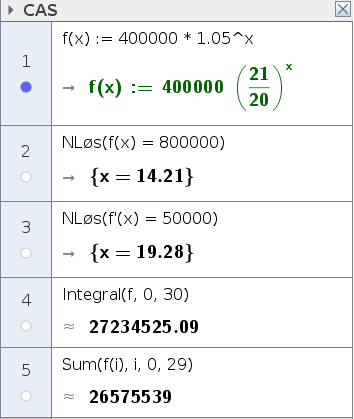
\includegraphics[width=0.45\linewidth]{figs/H17_del2_1bcde}
\caption{Utregninger for oppgave 1, del 2.}
\label{fig:H17_del2_1bcde}
\end{figure}

\subsection*{Oppgave 2}
\begin{easylist}[enumerate]
	\ListProperties(Style2*=,Numbers=a,Numbers1=l,FinalMark={)})
	# La oss innføre noen nyttige variabler:
	\begin{equation*}
		B = 1500000 \quad r = 1.003 \quad n = 180 \quad T = \text{ukjent terminbeløp}
	\end{equation*}
	Husk at i et annuitetslån så er alle terminbeløpene $T$ like.
	La $S(i)$ være skyldig beløp etter $i$ måneder.
	Da er 
	\begin{equation*}
		S(i) = S(i-1) \times r - T,
	\end{equation*}
	fordi skyldig beløp denne måneden er forrige skyldige beløp ganget med rentefaktoren $r$, minus terminbeløpet $T$.
	Vi kan sette opp en tabell som nedenfor.
	\begin{center}
		\begin{tabular}{ll}
			\textbf{Måned} $i$ & \textbf{Skyldig beløp} ($S(i)$)\\ \hline
			0 & $B$  \\
			1 & $Br - T$  \\
			2 & $(Br - T)r - T = Br^2 - T(1+ r)$  \\
			3 & $((Br - T)r - T)r - T = Br^3 - T(1+ r + r^2)$  \\
			$\vdots$ & $\vdots$ \\
			$n$ & $Br^n - T(1+ r + \dots + r^{n-1})$ 
		\end{tabular}
	\end{center}
	Etter $n$ år må det skyldige beløpet være lik null, vi får likningen
	\begin{equation}
	\label{eqn:Sn}
		S(n) = Br^n - T(1+ r + \dots + r^{n-1}) = 0.
	\end{equation}
	Vi bruker formelen for sum av en geometrisk rekke og skriver det som
	\begin{equation*}
	S(n) = Br^n - T \left[ \frac{1 - r^n}{1 - r} \right] = 0.
	\end{equation*}
	Denne likningen løser vi for $T$. Da får vi formelen
	\begin{equation*}
		T = \frac{B r^n (1 - r)}{1 - r^n},
	\end{equation*}
	som vi kan bruke til å finne $T$ med, som vist i figur \ref{fig:H17_del2_opp2a}.
	Svaret blir \answer{$T = 10 797$ kroner}. 
	På eksamen er det lurt å gjøre så mye som mulig i Geogebra, så istedet for å bruke formelen for summen av en geometriske rekke og løse likningen slik som ovenfor, kan det være lurt å løse likning \eqref{eqn:Sn} direkte i CAS.
	Dette er vist i figur \ref{fig:H17_del2_opp2a}, helt nederst.
	
	\begin{figure}[ht!]
	\centering
	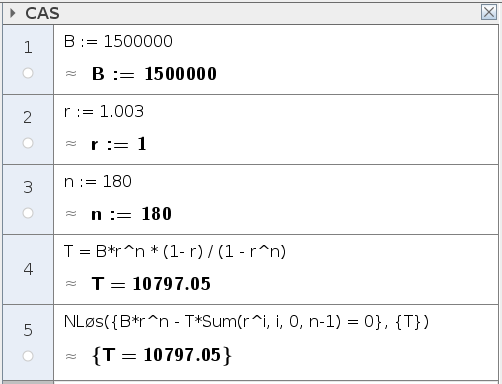
\includegraphics[width=0.6\linewidth]{figs/H17_del2_opp2a}
	\caption{Svar på oppgave 2a, del 2.}
	\label{fig:H17_del2_opp2a}
	\end{figure}

	# Denne oppgaven er rimelig lik forrige.
	Men nå er terminbeløpet kjent, og det skyldige beløpet $S(i)$ er ukjent.
	La oss kalle det kjente terminbeløpet for $T_1$, slik at $T_1 = 8000$ kroner.
	Vi kan sette opp en tabell som er lik den forrige.
	\begin{center}
		\begin{tabular}{ll}
			\textbf{Måned} $i$ & \textbf{Skyldig beløp} ($S(i)$)\\ \hline
			0 & $B$  \\
			1 & $Br - T_1$  \\
			2 & $(Br - T_1)r - T_1 = Br^2 - T_1(1+ r)$  \\
			3 & $((Br - T_1)r - T_1)r - T_1 = Br^3 - T_1(1+ r + r^2)$  \\
			$\vdots$ & $\vdots$ \\
			$n$ & $Br^n - T_1(1+ r + \dots + r^{n-1})$ 
		\end{tabular}
	\end{center}
	Vi må finne $S(n)$ når $n = 12 \times 5$.
	Se figur \ref{fig:H17_del2_oppg2b} for utregning i Geogebra,
	svaret blir \answer{$S(60) = $ 1270289 kroner}.
	
	\begin{figure}[ht!]
		\centering
		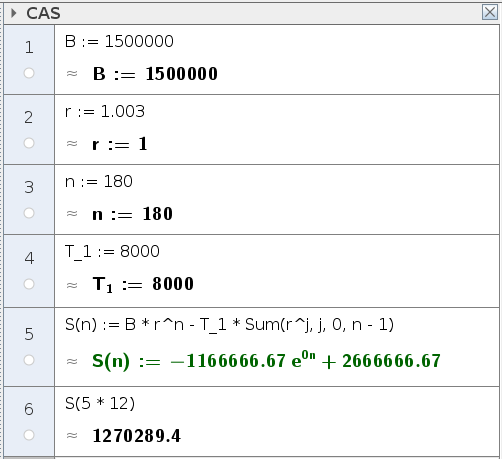
\includegraphics[width=0.625\linewidth]{figs/H17_del2_oppg2b}
		\caption{Svar på oppgave 2b, del 2.}
		\label{fig:H17_del2_oppg2b}
	\end{figure}
	
	# Denne oppgaven er helt lik første deloppgave, fordi vi er ute etter et ukjent terminbeløp $T$.
	Forskjellen er at nå er $B = 1270289$ og $n = 120$.
	Vi løser som vist i figur \ref{fig:H17_del2_2c}, og får 
	\answer{$T = 12621$ kroner} som terminbeløp for de resterende 120 månedene.
	
		\begin{figure}[ht!]
			\centering
			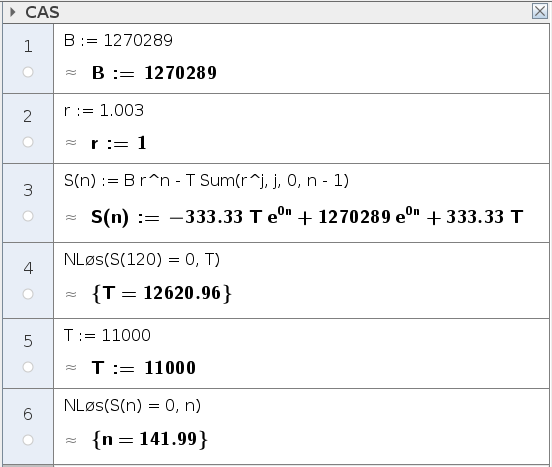
\includegraphics[width=0.65\linewidth]{figs/H17_del2_2cd}
			\caption{Svar på oppgave 2c og 2d, del 2.}
			\label{fig:H17_del2_2c}
		\end{figure}
	
	# Sett $T = 11000$ og løs for $n$.
	Vi får $n = 142$ som vist i figur \ref{fig:H17_del2_2c}.
	Tiden det tar å betale ned lånet går fra 120 måneder til 142 måneder, en \answer{økning på 22 måneder}.
	
	

\end{easylist}


\subsection*{Oppgave 3}
\begin{easylist}[enumerate]
	\ListProperties(Style2*=,Numbers=a,Numbers1=l,FinalMark={)})
	# Binomisk med $p = 0.85$ og $n = 200$.
	Vi bruker sannsynlighetskalkulatoren i Geogebra,
	og leser av at \answer{$P(X \geq 175) = 0.1876 \approx 18.8\%$}.
	
	# Vi skal undersøke
	\begin{align*}
		H_0 :  & \quad p = 0.85 \\
		H_1 :  & \quad p < 0.85 
	\end{align*}
	med signifikansnivå $5\%$. Vi observerer $X_\text{obs} = 160$.
	$P$-verdien er sannsynligheten for $P(X \leq X_\text{obs})$ gitt at $H_0$ er sann\footnote{At $H_0$ er sann betyr her at $p = 0.85$.}.
	Her er $P$-verdien lik 
	\begin{equation*}
		P(X \leq 160 \mid p = 0.85) = 0.0335,
	\end{equation*}
	og ettersom dette er mindre enn signifikansnivået \answer{forkaster vi $H_0$}.
	
	# Vi regner ut $\mu$ og $\sigma$ som
	\begin{align*}
		\mu &= np = 200 (0.85) = 170\\
		\sigma &= \sqrt{np(1-p)} = \sqrt{200 (0.85) (1 - 0.85)} = 5.0497524 \approx 5.05
	\end{align*}
	Vi regner ut $P(X \leq X_\text{obs})$ når $X$ er normaltfordelt, og vi må utføre korreksjon for heltallene slik at vi får
	\begin{equation*}
		P(X_\text{binom} \leq 160) \approx P(X_\text{norm} \leq 160.5).
	\end{equation*}
	Fra sannsynlighetskalkulatoren får vi at $P(X_\text{norm} \leq 160.5) = 0.02997 \approx 0.03$. 
	Vi \answer{forkaster $H_0$} ettersom $P$-verdien er mindre enn 5\%.
\end{easylist}

\end{document}


